\documentclass{report}

\usepackage{xcolor}
\usepackage{tikz}

\title{Poster designment}
\author{Weibin Zhang}
\date{Jun 8. 2018}
\begin{document}

Principle:
\begin{itemize}
    \item Constant font
    \item Multi-columns, allow spanning over a few nearby columns
	\begin{itemize}
	    \item customized column width
	\end{itemize}
    \item It depends on authors to fit their content into frames, rather
	than changing font size.
\end{itemize}

\begin{figure}[htb]
\centering
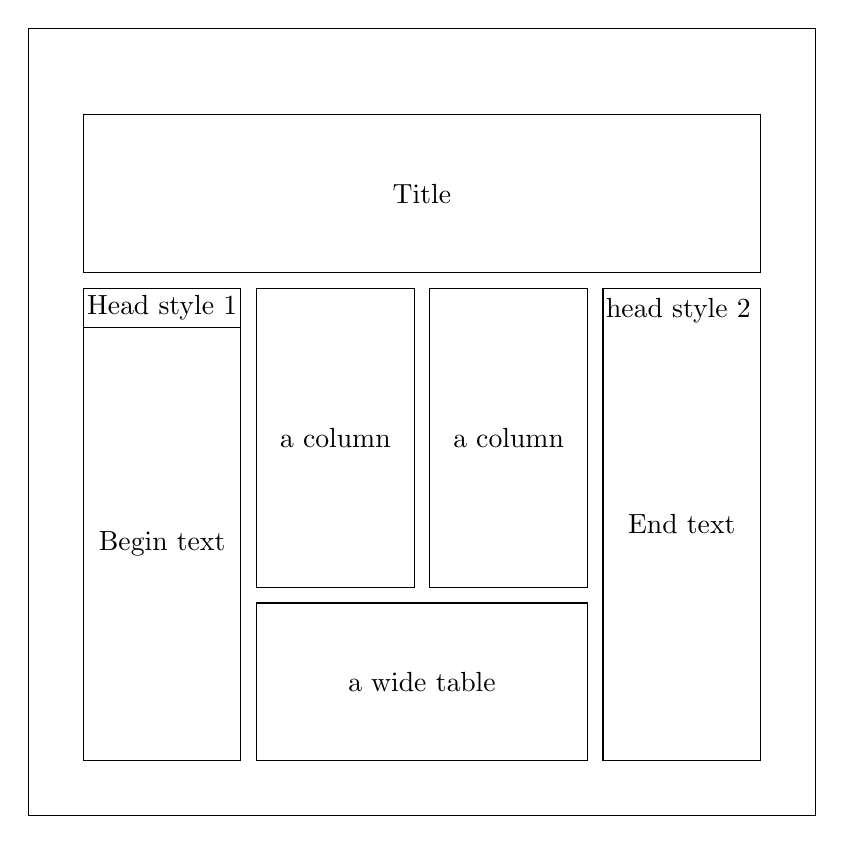
\begin{tikzpicture}
    \newlength{\posterinnersep}	    % inner seperation
    \setlength{\posterinnersep}{0.7cm}   
    \newlength{\posterxinnersep}    % horizontal inner seperation
    \setlength{\posterxinnersep}{0.7cm}   
    \newlength{\posteryinnersep}    % vertical inner seperation
    \setlength{\posteryinnersep}{0.7cm}   
    \newlength{\posterboxsep}	    % sepeartaion between boxes
    \setlength{\posterboxsep}{0.2cm}
    \newlength{\postercolsep}	    % column seperation
    \setlength{\postercolsep}{0.2cm}	    
    \newlength{\posterrowsep}	    % row seperation
    \setlength{\posterrowsep}{0.2cm}	    
    \draw (0, 0) rectangle (10, 10);
    \draw (\posterinnersep,\posterinnersep) rectangle node {Begin text} +(2, 5.5) 
	  ++(0, 5.5) rectangle node {Head style 1} +(2, 0.5);
    \draw (\posterinnersep + 2cm + \postercolsep,\posterinnersep + 0) rectangle node {a wide table} +(4.2, 2);
    \draw (\posterinnersep + 2cm + \postercolsep, \posterinnersep + 2cm + \postercolsep) rectangle node {a column} +(2, 3.8);
    \draw (\posterinnersep + 2*2cm + 2*\postercolsep, \posterinnersep + 2cm + \postercolsep) rectangle node {a column} +(2, 3.8);
    \draw (\posterinnersep + 3*2cm + 3*\postercolsep, \posterinnersep) rectangle node {End text} +(2, 6) node[anchor=north east] {head style 2};
    \draw (\posterinnersep ,\posterinnersep + \posterrowsep + 6cm) rectangle node {Title} +(8.6, 2);
\end{tikzpicture}
    \caption{An Example Poster Layout}
\end{figure}

\end{document}
